\DiaryEntry{Upcoming Ideas...}{}{}

\subsection{Making a denominator square-root free.}

\bee
\frac{1}{1 + \sqrt{2}} = \frac{1 - \sqrt{2}}{(1 + \sqrt{2})(1 - \sqrt{2})} = \frac{1 - \sqrt{2}}{1 - 2} = \sqrt{2} - 1
\eee

Based on $(a-1)(a+1) = a^2 - 1$.

A similar idea is to make the denominator real,

\bee
\frac{1}{1-j} = \frac{1+j}{(1-j)(1+j)} = \frac{1+j}{(1-j)(1+j)} = \frac{1+j}{2}
\eee


\subsection{Graph / Tree traversal}

Actually, two things. Numerb one: The DFS algorithm \ref{2020-02-27:entry} is recursive. There is, however, also an iterative version available which uses a stack. Implement this algorithm.

Number two: Both BFS and DFS simplify in case of a tree as it is a graph without cycles. Show how the algs simplify in this case.


\subsection{Inequalities and Squareroots}

Prove that $0 < 11 - 6 \sqrt{3} < 1$. We have the following reasoning:

\begin{align*}
  &121 > 108 > 100 \\
  &\sqrt{121} > \sqrt{108} > \sqrt{100} \\
  &11 > 6 \sqrt{3} > 10 \\
  &-11 < -6 \sqrt{3}  < -10
\end{align*}

The square root is a convex function, therefore from $A > B$ follows $\sqrt{A} > \sqrt{B}$ which explains the step from the first to second line.

Adding $11$ to the last line yields

\bee
0 < 11 - 6 \sqrt{3} < 1 \qed
\eee

Also interesting is to bound a square root between integers which differ by one; e.g. $A < \sqrt{37} < B$. We can bound this as follows

\begin{align*}
  &\sqrt{36} < \sqrt{37} < \sqrt{49} \\
  & 6 < \sqrt{37} < 7
\end{align*}

For the lower / upper bound we use the ``closest'' square number. The root then gives integers and the bounds differ by $1$ as requested. This holds for all numbers in between; i.e. we have

\bee
6 < \sqrt{37} \cdots \sqrt{48} < 7
\eee


\subsection{Distance Point - Random Point}

Here we have one fixed point $P(x_P,0)$ and ask for the distance $d$ to another point $Q$ located randomly inside the unit circle / box. The distance $d$ is random and given by

\bee
d = \sqrt{(x_p - x)^2 + y^2}
\eee

where $(x,y)$ are the coordinates of $Q$. In case of a unit box, they are distributed according to

\bee
x,y \sim \Uc(-1,1)
\eee

in case of a unit circle, they are constrained by $x^2 + y^2 \leq 1$. According to \href{https://stats.stackexchange.com/questions/481543/generating-random-points-uniformly-on-a-disk}{this} Stackoverflow answer, the distributions of $x$ and $y$ are a bit more tricky...

The expected distance $E(d)$ is then given by

\bee
E(d) = \int_{x,y} d f_x(x) f_y(y) dx dy
\eee

where $f_x(x), f_y(y)$ are the distributions of $x$ and $y$, respectively. The integrals seem to be rather tricky; even in case of the unit box (where the distribution is simple), I'm not sure if there is a closed-form solution for the double-integral. In case of the unit disc, already the distributions are complex (polar coordinates may help as $\phi$ is uniform in $[0, 2\pi]$ and $r$ is $\sim  r$ in $[0,1]$.

\subsection{Predator-Prey}

See entry \ref{2018-07-30:entry} and extend it to general coefficients,

\begin{align}\label{2018-07-30-eq1}
R' = \frac{dR}{dt} &= \alpha R - \beta RF \nonumber \\
F' = \frac{dF}{dt} &= -\gamma F + \delta RF
\end{align}

We can rewrite the first equation as $R(\alpha - \beta F) = 0$ and obtain two fixed points from it: (i) $R = $, (ii) $F = \alpha/\beta$. We can use the second equation similarly, $F(- \gamma+  \delta R)$ and obtain (i) $F = 0$, (ii) $R = \gamma/\delta$. Therefore, we have two fixed points,

\begin{align}
  &R = F = 0\\
  &R = \gamma / \delta, F = \alpha / \beta
\end{align}

To assess the stability of the fixed points, we calculate the Jacobian $\Jbf$ of the differential equation system \todo{Check!!!},

\bee
\Jbf = \begin{pmatrix} \frac{dR'}{dR} & \frac{dR'}{dF} \\ \frac{dF'}{dR} & \frac{dF'}{dF} \end{pmatrix} = \begin{pmatrix} \alpha - \beta F & - \beta R \\ \delta F & \delta R - \gamma \end{pmatrix}
\eee

Let's consider the fixed point $R = F = 0$ first. For these values, the Jacobian becomes

\bee
\Jbf_1 = \begin{pmatrix} \alpha & 0 \\ 0 & - \gamma \end{pmatrix}
\eee

The eigenvalues are the solution to $|\Jbf_1 - \lambda \Ibf | = 0$. We have

\bee
\begin{vmatrix} \alpha - \lambda & 0 \\ 0 & - \gamma - \lambda \end{vmatrix} = (\alpha - \lambda)(- \gamma - \lambda) = 0
\eee

and therefore the two eigenvalues become $\lambda_1 = \alpha, \lambda_2 = - \gamma$. In our model, the parameters $\alpha$ and $\gamma$ are always greater than zero, and therefore such the sign of the eigenvalues will be different. Hence the fixed point at the origin is a saddle point which is an instable fixed point \todo{is a saddle point always instable?}.

For the other fixed point ($R = \gamma / \delta, F = \alpha / \beta$), the Jacobian becomes

\bee
\Jbf_2 = \begin{pmatrix} \alpha - \beta \alpha / \beta & - \beta \gamma / \delta \\ \delta \alpha / \beta & \delta \gamma / \delta - \gamma \end{pmatrix} = \begin{pmatrix} 0 & - \beta \gamma / \delta \\ \delta \alpha / \beta & 0 \end{pmatrix}
\eee

The eigenvalues of this matrix are given by

\bee
\begin{vmatrix} -\lambda & - \beta \gamma / \delta \\ \delta \alpha / \beta & - \lambda \end{vmatrix} = \lambda^2 - (- \beta \gamma / \delta)(\delta \alpha / \beta) = 0
\eee

From this follows

\bee
\lambda^2 + \alpha \gamma = 0 \rightarrow \lambda_{1,2} = \pm j \sqrt{\alpha \gamma}
\eee

As the eigenvalues are both purely imaginary and conjugate to each other, this fixed point must either be a center for closed orbits in the local vicinity or an attractive or repulsive spiral. In conservative systems, there must be closed orbits in the local vicinity of fixed points that exist at the minima and maxima of the conserved quantity. \todo{Copied from Wikipedia - do not understand completely!}

\begin{figure}[H]
    \centering
    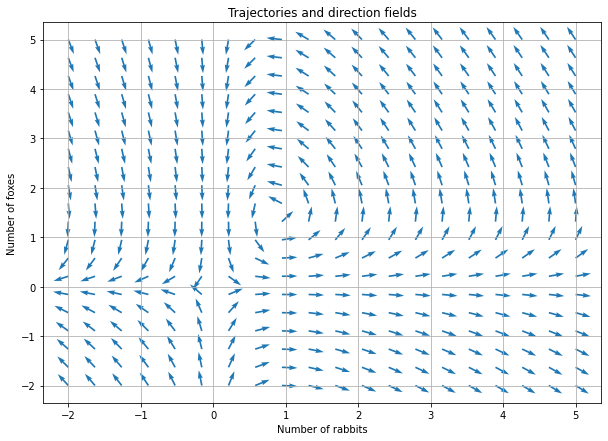
\includegraphics[scale=0.6]{images/predator_prey.png}
\end{figure}


\subsection{Walli's Integral}

Defined as (Nahin, Inside Interesting Integrals, p. 122),

\bee
I(k) = \int_0^1 (x-x^2)^k dx = \int_0^1 x^k (1-x)^k dx = B(k+1, k+1) = \frac{\Gamma(k+1) \Gamma(k+1)}{\Gamma(2k+2)}
\eee

which becomes (for integer-valued $k$)

\bee
I(k) = \int_0^1 (x-x^2)^k dx = \frac{(k!)^2}{(2k+1)!}
\eee

Especially interesting is $k =1/2$. TODO


\subsection{Integral $\log(x)/x^k$}

Start with $k = 2$ and consider the following integral

\bee
I = \int_1^\infty \frac{\log(x)}{x^2}dx
\eee

which we can solve via partial integration: We chose $u=\log(x), v'=1/x^2$ and obtain $u' = 1/x, v = -1/x$ and therefore the integral becomes

\bee
I = - \left. \frac{\log(x)}{x} \right|_1^\infty + \int_1^\infty \frac{1}{x^2} dx = 0 + \left.\left( - \frac{1}{x} \right)\right|_1^\infty = 1
\eee

Interestingly, this can be extended to

\bee
I = \int_1^\infty \frac{\log(x)}{x^k}dx
\eee

Same procedure, $u=\log(x), v'=1/x^k$ and obtain $u' = 1/x, v = \frac{x^{-k+1}}{-k+1}$ and therefore we have

\bee
I = - \left. \frac{x^{-k+1} \log(x)}{-k+1} \right|_1^\infty - \int_1^\infty x^{-1} \frac{x^{-k+1}}{-k+1} dx = 0 - \frac{1}{1-k} \int_1^\infty x^{-k} dx = \frac{1}{(k-1)^2}
\eee

\subsection{Where should I open my restaurant?}

Based on \cite{Kaplan2017}.

A walk on the $\Zc^2$ lattice using only the steps $(0, 1)$, which we call ``North'', and $(1, 0)$, which we call ``East'' is a lattice path.

Question 1: How many lattice paths begin at $(0, 0)$ and end at $(m, n)$?

The path consists of $m$ steps East and $n$ steps North. In total we need to make $m+n$ steps to reach the destination and it does not matter when we go North and East. We therefore have

\bee
{m+n \choose m}
\eee

different lattice paths. A classical application of the binomial.

Question 2: How many of these paths pass through the point $(a, b)$?

We can split the path into two parts: One from $(0,0)$ to $(a,b)$ and one from $(a,b)$ to $(m,n)$. We can apply the same argument from before to each of the two paths and note that we can chose them independently; i.e. we multiply their numbers.

For the first part we have ${a+b \choose a}$ possibilities, for the second one (with $m-a$ steps East and $n-b$ steps North) we have ${m-a+n-b \choose m-a}$ possibilities. Therefore, there are

\bee
{a+b \choose a} {m-a+n-b \choose m-a}
\eee

different lattice paths.

\subsection{TIKZ}

Some text...

\begin{figure}[H]
\centering
\begin{tikzpicture}[transform shape]
  \graph [nodes={circle,draw}] {
    %A -> ["1"] B -> ["2"] C;
    %D -> ["4"] C;
    A -> ["1"] B -> ["2"] C;
    D -> ["4"] C;
    A ->["3", bend left] C;
  };
\end{tikzpicture}
\caption{Example Graph, I.}
\end{figure}



%%% Local Variables:
%%% mode: latex
%%% TeX-master: "journal"
%%% End:
